\section{LDAを用いた物体のトピック分類}
物体のトピック分類を行うためにトピックモデリング手法の1つであるLDA\cite{lda}を用いる.
LDAではパラメータ$\alpha$と$\beta$を用いてドキュメントが生成されると仮定する.
これを表したLDAのグラフィカルモデルは以下のようになる.
\begin{figure}[h!]
	\begin{center}
		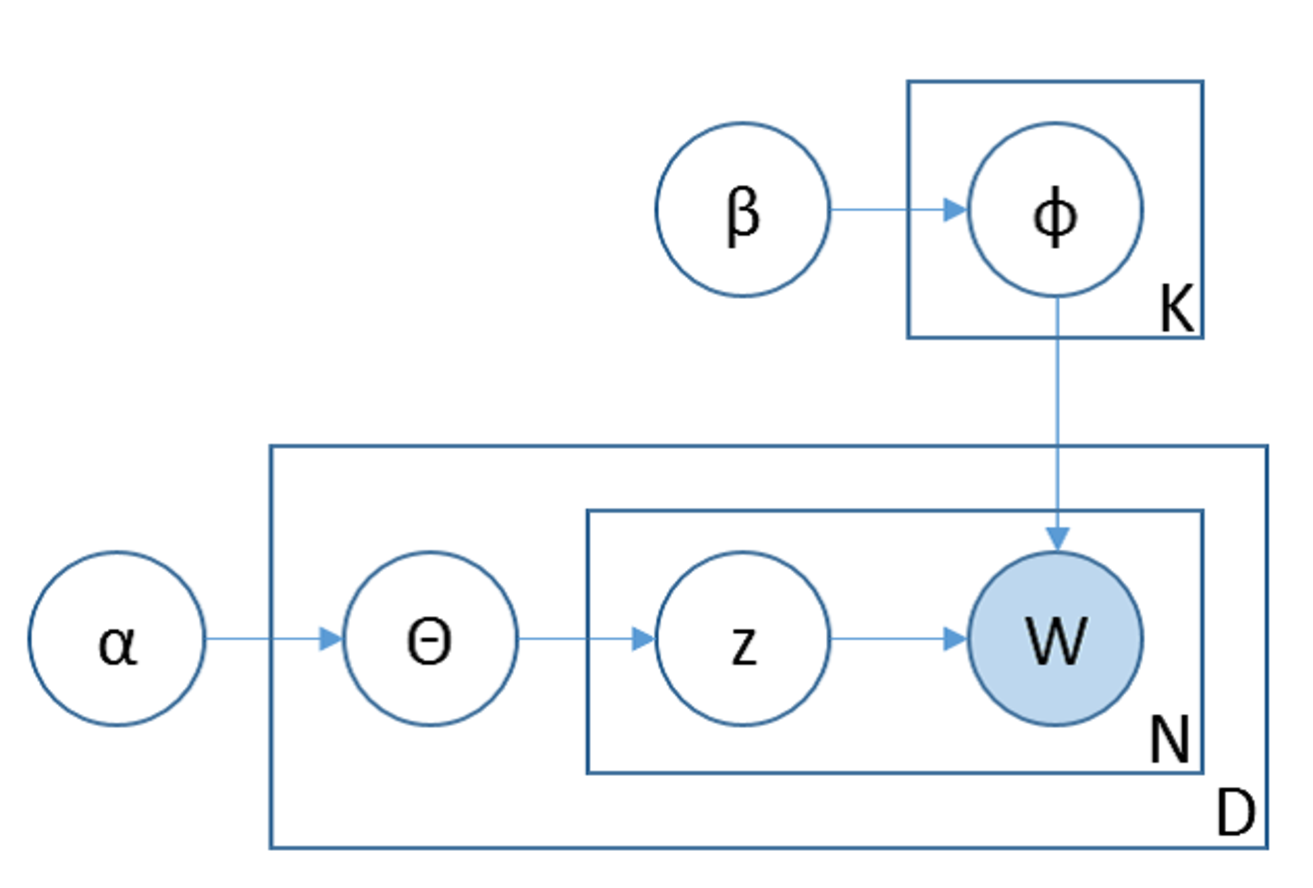
\includegraphics[width=0.25\textwidth,clip]{img/graphicalmodel.eps}
	\end{center}
	\caption{LDAにおけるグラフィカルモデル}
	\label{fig:graphical_model}
\end{figure} 
\begin{figure}[h!]
	\begin{minipage}[b]{0.5\linewidth}
		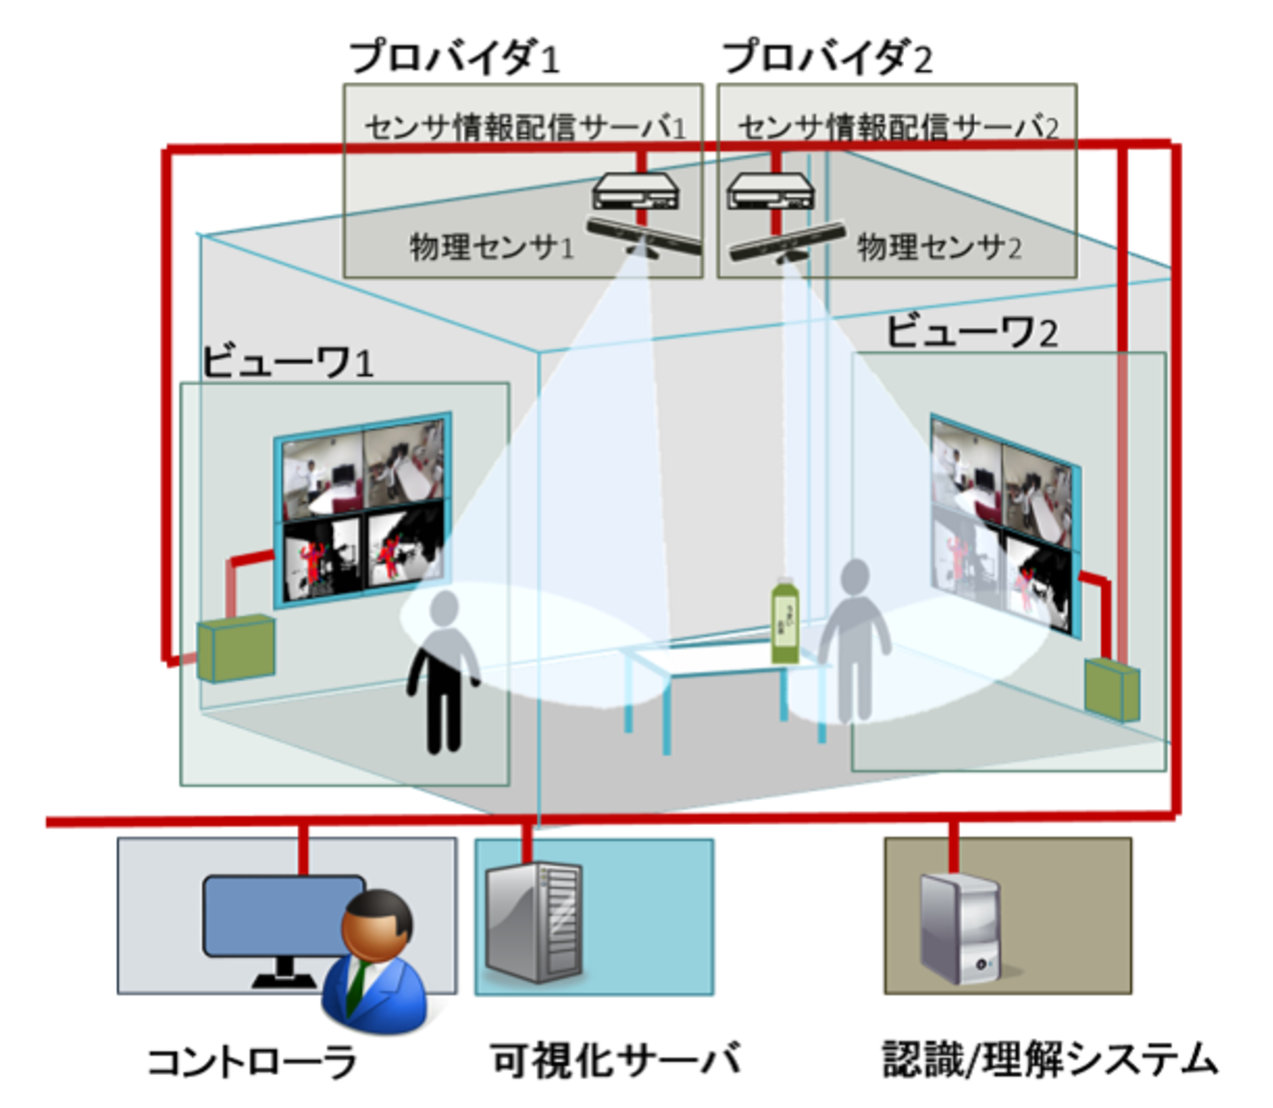
\includegraphics[width=\textwidth,clip]{img/infra.eps}
		\caption{ネットワーク指向型センサ/ディスプレイ基盤}
		\label{fig:infra}
        \end{minipage}%
	\begin{minipage}[b]{0.5\linewidth}
		\includegraphics[width=0.9\textwidth,clip]{img/viewer.eps}
		\caption{複数センサからの情報の閲覧}
		\label{fig:infra}
        \end{minipage}
\end{figure}

\par
%グラフィカルモデルにおける単語は入力画像をBag of Feature(BoF)によって表現する.
LDAのグラフィカルモデルにおける1ドキュメントは1画像に該当し, 
1画像の中に現れる局所特徴をBag of Feature(BoF)で表現したものが単語に該当する.
具体的には, 128次元のSIFT\cite{sift}を用いて変換した後, 
K平均法\cite{kmeans}を用いてベクトル量子化し, $T$個のクラスに分けたヒストグラムを用いる.
\par
このような画像から作成したドキュメントの集合とトピック数$K$を入力とする.
学習にはギブスサンプラーを用いてトピックの事後分布から$z$をサンプリングする(式(\ref{gibbs})).
\begin{equation}
p(z = t|w, d) \propto ( \alpha_{t} + n_{t|d} ) \frac{\beta + n_w}{\beta V + n_t}
\label{gibbs}
\end{equation}
\par


